\documentclass{standalone}
\usepackage{tikz}
\usepackage{pgfplots}
\usetikzlibrary{intersections,positioning,calc,patterns}
\usepackage{lmodern}
\usepackage[T1]{fontenc}
\begin{document}
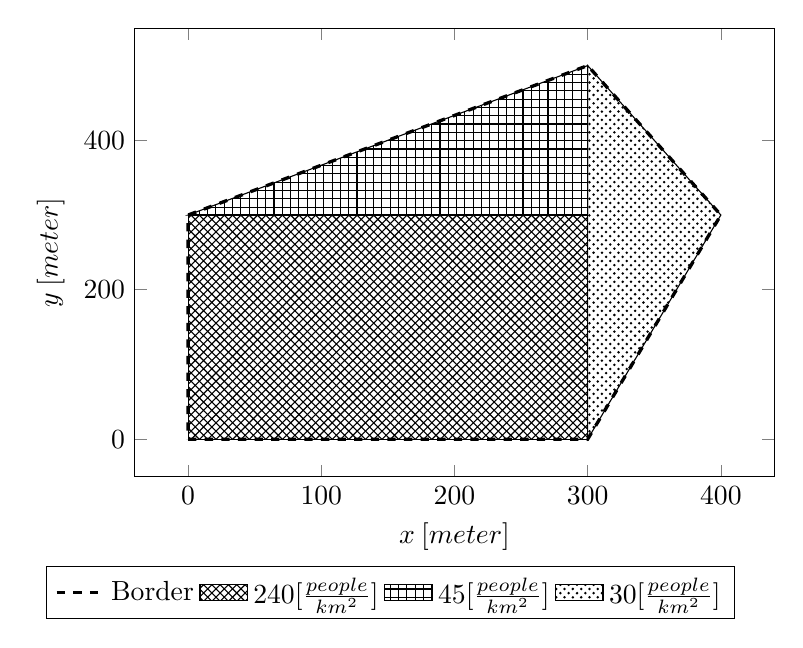
\begin{tikzpicture}
    \begin{axis}[
	width=0.8\textwidth,
      height=0.6\textwidth,
        xlabel={ $x\:[meter]$},
        ylabel={ $y\:[meter]$},
        legend style={at={(0.4,-0.2)},
      anchor=north,legend columns=-1}]
   
    \addplot+[mark=none,draw=black, very thick,dashed] coordinates 
		{(0,0) (300,0) (400,300) (300,500) (0,300)} -- cycle;
    \addlegendentry{Coverage area} 
    
     \addplot+[mark=none,pattern=crosshatch,area legend,draw=black] coordinates 
		{(0,0) (300,0) (300,300) (0,300)} -- cycle;
    	\addlegendentry{240$[\frac{people}{km^2}]$}
    	
    	\addplot+[mark=none,pattern=grid,area legend,draw=black] coordinates 
		{(0,300) (300,300) (300,500) (0,300) } -- cycle;
    	\addlegendentry{45$[\frac{people}{km^2}]$}
    	
    	\addplot+[mark=none,pattern=crosshatch dots,area legend,draw=black] coordinates 
		{(300,0) (300,500) (400,300) }-- cycle;
    	\addlegendentry{30$[\frac{people}{km^2}]$}
		\legend{Border,240$[\frac{people}{km^2}]$,45$[\frac{people}{km^2}]$,30$[\frac{people}{km^2}]$}
    \end{axis}
\end{tikzpicture}
\end{document}